 % -----------------------------------------------
% Template for SMC 2009
%     smc2009.sty -> style file
% Last modified by Fabien Gouyon (smc2009@inescporto.pt)
% Modified by Juan P. Bello (ismir2008-papers@ismir.net)
% By Rainer Typke (ismir07.rainer@safersignup.com)
% Based on the 2004 template by Eloi Batlle.
% -----------------------------------------------

\documentclass{article}
\usepackage{stsm2009,amsmath}
% To use when using pdflatex
\usepackage{graphicx}
\usepackage{url}     
\usepackage{hyperref}  
      
\newenvironment{packed_item}{
\begin{itemize}
  \setlength{\itemsep}{1pt}
  \setlength{\parskip}{0pt}
  \setlength{\parsep}{0pt}
}{\end{itemize}}

\newenvironment{packed_enumerate}{
\begin{enumerate}
  \setlength{\itemsep}{1pt}
  \setlength{\parskip}{0pt}
  \setlength{\parsep}{0pt}
}{\end{enumerate}}
% To use when using latex, dvips and ps2pdf
% \usepackage[dvips]{graphicx}


\title{ADVANCED REAL-TIME CONTROL OF PARAMETERS \\BY INTEGRATION OF JAMOMA AND FTM IN MAX.\\
Report of a COST IC0601 SID Short-Term Scientific Mission April 2009 \\Hosted by The Real-Time Musical Interactions Team, IRCAM, Paris (FR)}
% IMPORTANT NOTICE:
% Reviews are double-blind
% Authors will not be informed of who reviews their papers, and author names will be concealed from the reviewers 
% Please avoid evident self references in the text

% Authors' names must be omitted from title page (or listed as �name(s) omitted for submission�)


% Single address
% To use with only one author or several with the same address
% ---------------
\oneauthor
   {Trond Lossius} {BEK - Bergen Center for Electronic Arts \\ Bergen (NO) \\ trond.lossius@bek.no} 
 


% Two addresses
 %--------------
%\threeauthors
%  {First author} {School \\ Email}
%  {Second author} {Company \\ Email}
%  {Third author} {Company \\ Email}
% Three addresses
% --------------
%\threeauthors
%  {First author} {School \\ Email}
%  {Second author} {Company \\ Email}
%  {Third author} {Company \\ Email}

\begin{document}
%    
\sloppy
\maketitle
%

\permission

\begin{abstract}  



\end{abstract}

\section{Introduction}\label{sec:introduction}         


%%%%%%%%%%%%%%%%%%%%%%%%%%%%%%%%%%%%%%%%%%%%%%%%%%%%%%%%%%%%%%%%%%%%%%%%%%%%%
%
%%%%%%%%%%%%%%%%%%%%%%%%%%%%%%%%%%%%%%%%%%%%%%%%%%%%%%%%%%%%%%%%%%%%%%%%%%%%%

\section{A section}  
 



%%%%%%%%%%%%%%%%%%%%%%%%%%%%%%%%%%%%%%%%%%%%%%%%%%%%%%%%%%%%%%%%%%%%%%%%%%%%%
%
%%%%%%%%%%%%%%%%%%%%%%%%%%%%%%%%%%%%%%%%%%%%%%%%%%%%%%%%%%%%%%%%%%%%%%%%%%%%%

\section{A section}   


%%%%%%%%%%%%%%%%%%%%%%%%%%%%%%%%%%%%%%%%%%%%%%%%%%%%%%%%%%%%%%%%%%%%%%%%%%%%%
%
%%%%%%%%%%%%%%%%%%%%%%%%%%%%%%%%%%%%%%%%%%%%%%%%%%%%%%%%%%%%%%%%%%%%%%%%%%%%%

\section{Discussion \& Conclusion}



%%%%%%%%%%%%%%%%%%%%%%%%%%%%%%%%%%%%%%%%%%%%%%%%%%%%%%%%%%%%%%%%%%%%%%%%%%%%%
%
%%%%%%%%%%%%%%%%%%%%%%%%%%%%%%%%%%%%%%%%%%%%%%%%%%%%%%%%%%%%%%%%%%%%%%%%%%%%%

\section{Acknowledgment}

 The COST IC0601 Action on Sonic Interaction Design (SID) .


\bibliographystyle{abbrv}  %\bibliographystyle{natbib}% ama, nar, alpha, plain, chicago,{plainnat}  abbrv, siam   
\small
\bibliography{stsm09}
\end{document}   



% \section{Style Stuff - delme}

% \subsection{Title and Authors}

%The title is 14pt Times, bold, caps, upper case, centered. Authors' names are centered. 
%The lead author's name is to be listed first (left-most), and the co-authors' names after. If the addresses for all 
%authors are the same, include the address only once, centered. If the authors have different addresses, 
%put the addresses, evenly spaced, under each authors' name.

% Reviews are double-blind. {\it \textbf{Author information should be removed from this page in initial submissions}}, 
% and only added later by the authors when sending camera-ready versions.

%\subsection{Figures, Tables and Captions}

%All artwork must be centered, neat, clean, and legible. All lines should
%be very dark for purposes of reproduction and art work should not be hand-drawn.
%The proceedings is not in color, and therefore all figures must make
%sense in black-and-white form.
%Figure and table numbers and captions always appear below the figure. Leave 1
%line space between the figure or table and the caption. Each figure or table
%is numbered consecutively. Captions should be Times 10pt.
%Place tables/figures in text as close to the reference as possible.
%References to figures and tables should be capitalised, for example:
%see Figure \ref{fig:example} and Table \ref{tab:example}.
%Figures and tables may extend across both columns to a maximum
%width of 7'' (17.78~cm).

%\begin{table}
%\begin{center}
%\begin{tabular}{|l|l|}
%\hline
%String value & Numeric value \\
%\hline
%hello SMC  & 1073 \\
%\hline
%\end{tabular}
%\end{center}
%\caption{Table captions should be placed below the table}
%\label{tab:example}
%\end{table}

%\begin{figure}
%\centerline{\framebox{
% To use when using pdflatex
%	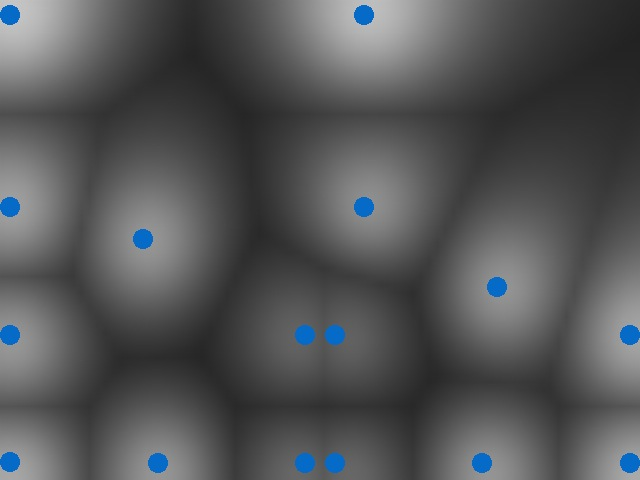
\includegraphics[width=\columnwidth]{../ICMC2009-dbap/all_r_6_b_0_2}}}
	% To use when using latex, dvips and ps2pdf
% 	
\includegraphics[width=\columnwidth]{figure.eps}}}
%\caption{Figure captions should be placed below the figure}
%\label{fig:example}
%\end{figure}